\section{Use-Case Modellierung}
\label{sec:use-case-modellierung}

% Use-Case(s) (-> functional requirements)
% Veränderungen zwischen bestehender und Cloud nativer Anwendung
% -> Beeinflussen von functional requirements

\subsection{Use-Case Definition}
Der für den Prototypen ausgewählte Use-Case ist das \glqq{Einsammeln}\grqq der Timesheets. Aus einer Konfigurationsdatei hinaus soll festgelegt werden für welches Projekt und welchen Zeitraum diese von dem Projektverzeichnis in ein temporäres Verzeichnis kopiert werden sollen. Nachfolgend wird der Use-Case definiert, um im Anschluss an die Implementierung untersuchen zu können, ob dieser auch nach der Migration in die Cloud erfüllbar ist. % Unter diesem Haupt-Use-Case definieren sich weitere Sub-Use-Cases, die wie folgt aussehen:
% \begin{itemize}
% \item \textbf{Einlesen der Konfigurationsdatei:} Lesen der Parameter für Box-Zugriff und Projektdaten aus der Konfigurationsdatei
% \item \textbf{Lesen des PMO Files:} Lesen des Projektmanagement-Files aus dem Box-Verzeichnis zur Ermittlung der Namen aktiver Mitarbeiter
% \item \textbf{Einsammeln (Kopieren) der Timesheets:} Erfassen der Timesheets aller aktiven Mitarbeiter und Kopieren dieser in das temporäre Verzeichnis
% \end{itemize}
\begin{table}[H]
    \begin{tabular}[H]{|l|l|}
        \hline
        \multicolumn{2}{|l|}{\textbf{Anwendungsfall:} Einsammeln der Timesheets} \\
        \hline
        \textbf{Kurzbeschreibung:} & Timesheets aktiver Mitarbeiter in temporäres Verzeichnis kopieren \\
        \hline
        \multicolumn{2}{|l|}{\textbf{Normalverlauf}} \\
        \hline
        \multicolumn{2}{|l|}{1. Leeren des temporären Ordners} \\
        \multicolumn{2}{|l|}{2. PMO Datei finden und laden} \\
        \multicolumn{2}{|l|}{3. Aktive Mitarbeiter aus PMO Datei lesen} \\
        \multicolumn{2}{|l|}{4. Timesheets der aktiven Mitarbeiter kopieren} \\
        \hline
        \multicolumn{2}{|l|}{\textbf{Alternativablauf}} \\
        \hline
        \multicolumn{2}{|l|}{Siehe Normalverlauf} \\
        \multicolumn{2}{|l|}{\textbf{Qualitätsanforderungen}} \\
        \hline
        \multicolumn{2}{|l|}{1. Für jeden aktiven Mitarbeiter soll ein Timesheet im temporären Ordner liegen} \\
        \multicolumn{2}{|l|}{2. Die Timesheets sollen unverändert sein (Dateiname, Inhalt)} \\
        \multicolumn{2}{|l|}{3. Eigener Zielordner pro Monat zur Vermiedung von Vermischungen} \\
        \multicolumn{2}{|l|}{4. Die Timesheet Größe kann variieren -> keine Limitierungen} \\
        \multicolumn{2}{|l|}{5. Es darf keine Kompression mit Formatänderung eingesetz werden} \\
        \multicolumn{2}{|l|}{6. Ein Logfile soll Erfolg und Misserfolg von Kopiervorgängen enthalten} \\
        \multicolumn{2}{|l|}{7. Fehlersituationen auf einzelnen Dateien dürfen den Ablauf nicht unterbrechen} \\
        \multicolumn{2}{|l|}{8. Root-Verzeichnisse für Ziel und Quelle müssen konfigurierbar sein} \\
        \hline
    \end{tabular}
    \caption{Anwendungsfall: Einsammeln der Timesheets}
    \label{tab:use-case-analyse-timesheets}
\end{table}

\begin{figure}[H]
    \centering
    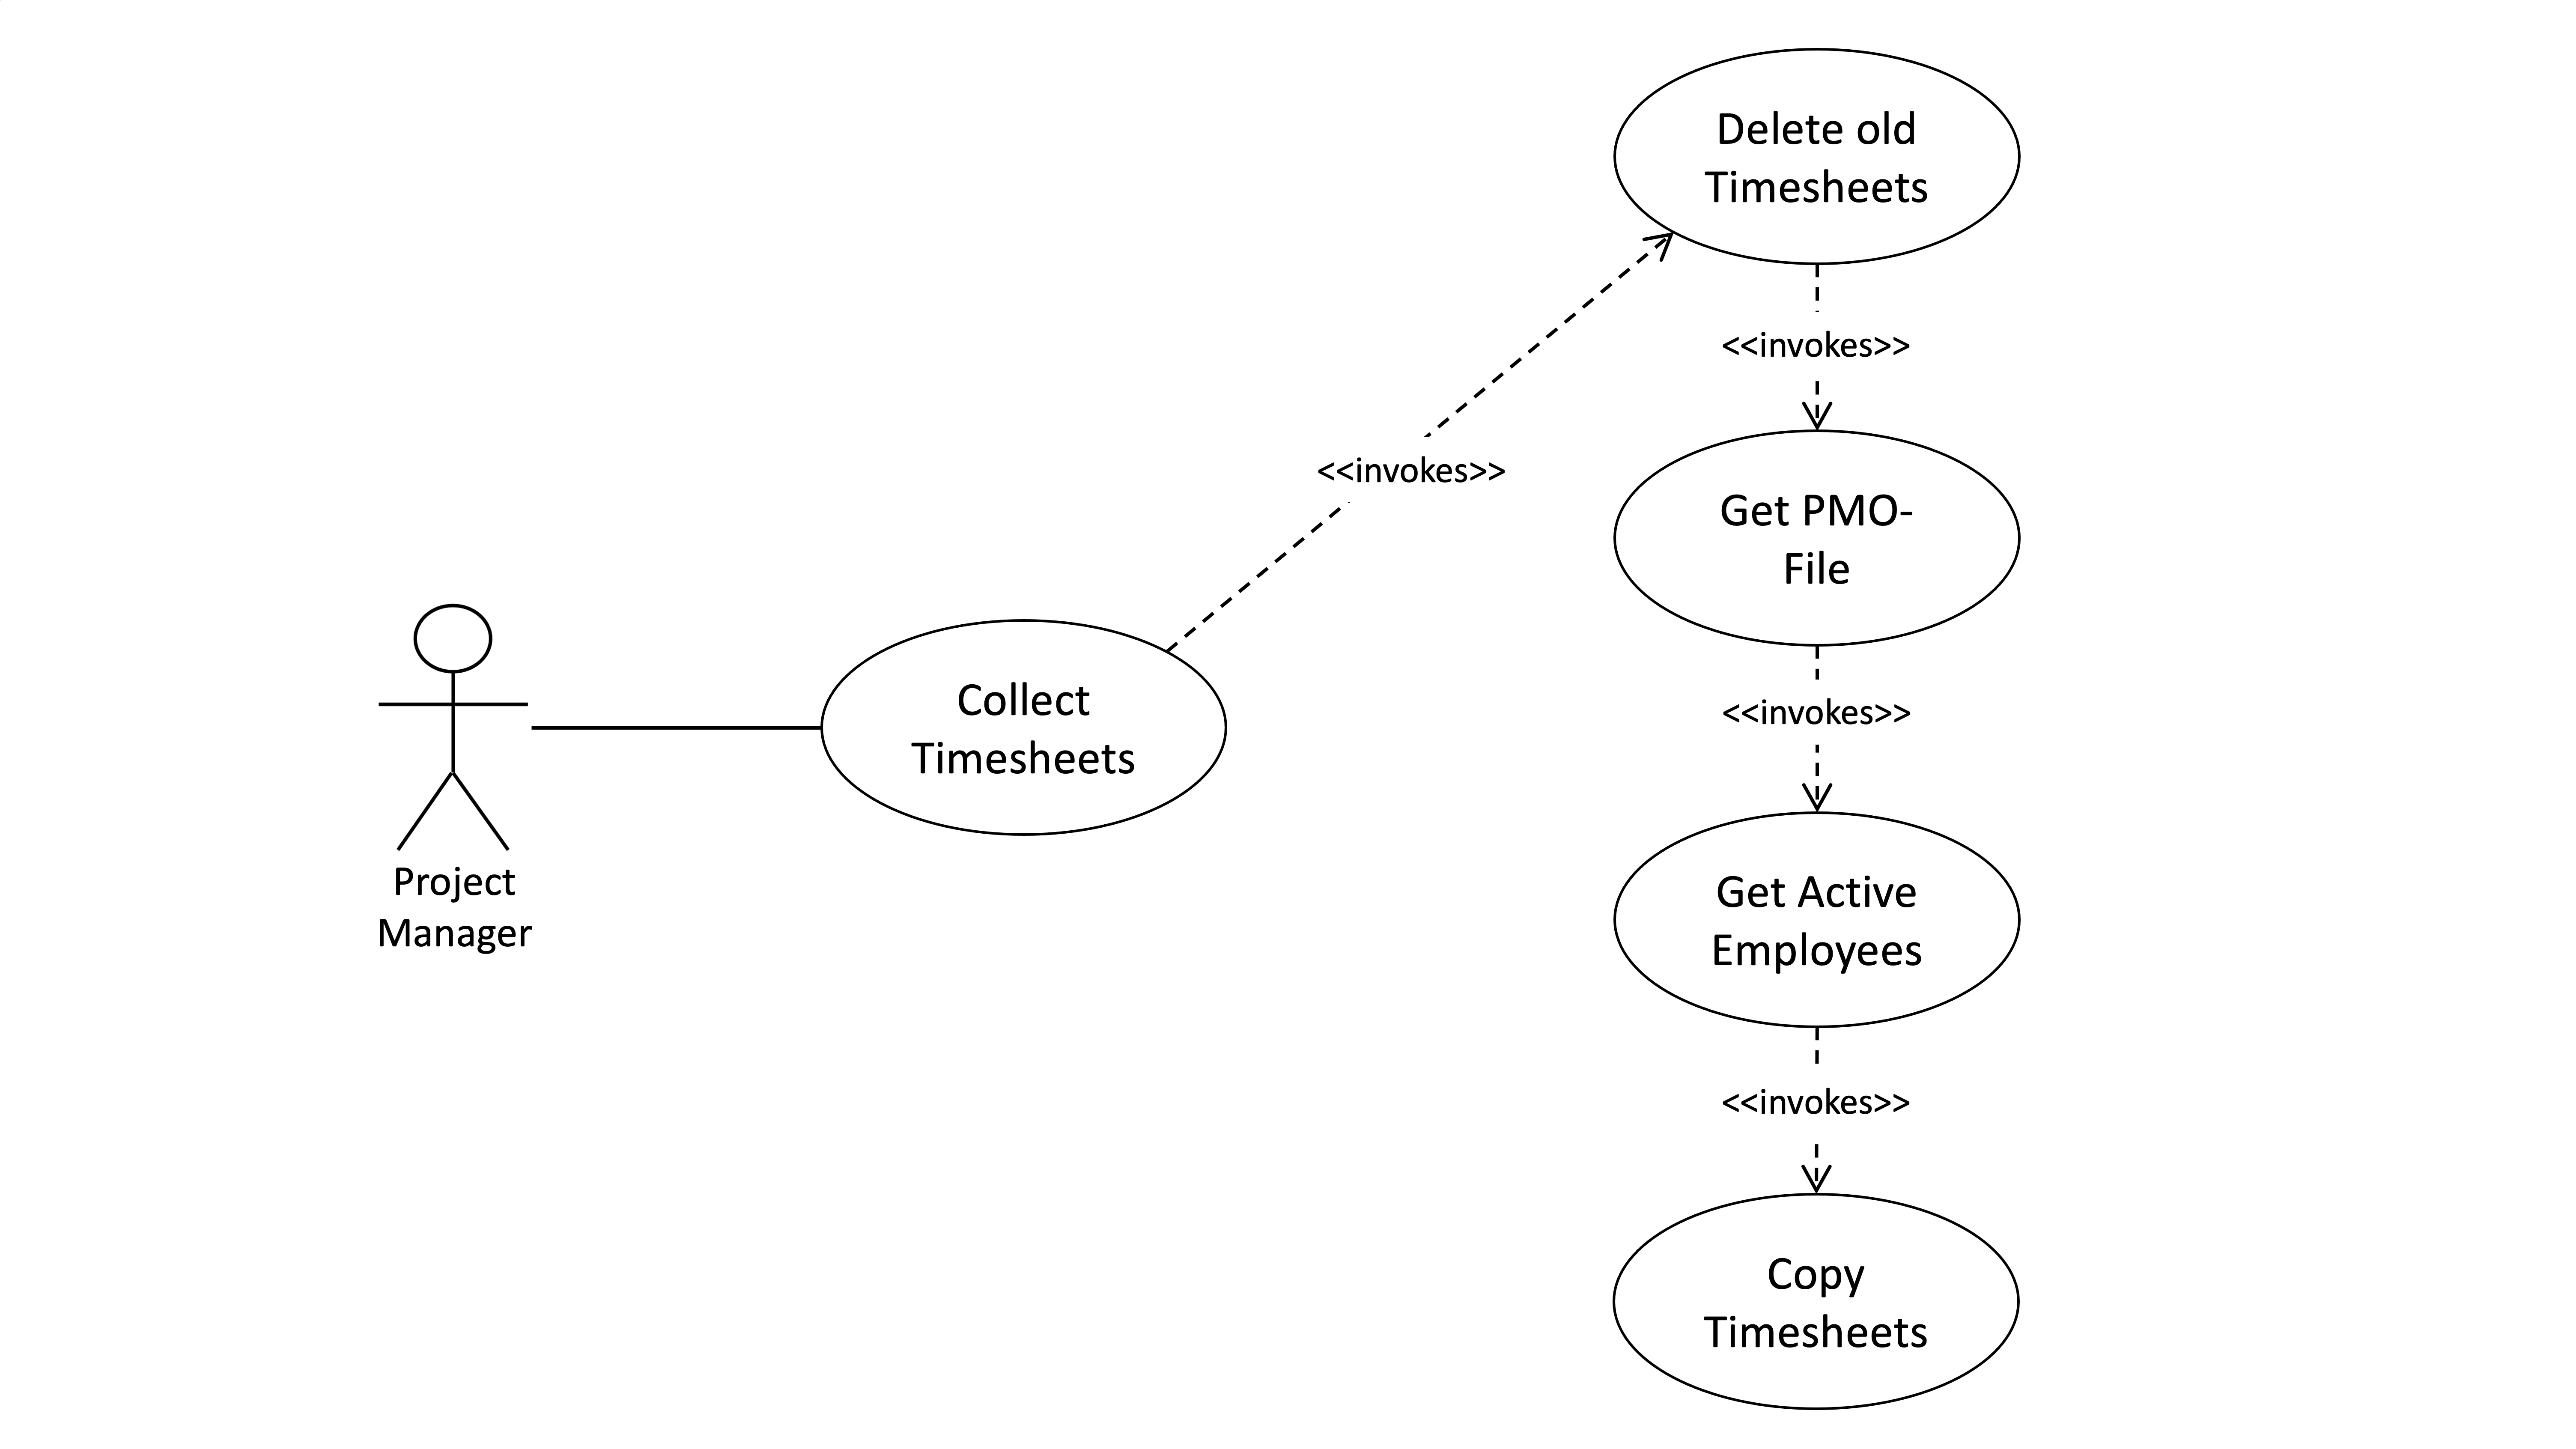
\includegraphics[width=\textwidth]{use-case-diagram.png}
    \caption{Use-Case Diagramm}
    \label{fig:use-case-diagram}
\end{figure}

Anschließend an diesen Prozess würden die weiteren Services der Toolsuite folgen, die für den Umfang dieser Arbeit ausgelassen wurden.
